%---------------------------------------------------------------------
% Course    : Introduction To web sciences
% Professor : Dr.Nelson
% Name      : Babitha Bokka
% Assignment: 7
%---------------------------------------------------------------------
\documentclass[12pt]{article}
%--------------------------------------------------------------------
% packages required
%--------------------------------------------------------------------
\usepackage{graphicx}
\usepackage{listings}
\usepackage{hyperref}
\usepackage{caption}
\usepackage{color}
\usepackage{pdfpages}
\graphicspath{ {images/} }
%--------------------------------------------------------------------
% Start Margins
%--------------------------------------------------------------------
\addtolength{\oddsidemargin}{-.875in}
\addtolength{\evensidemargin}{-.875in}
\addtolength{\textwidth}{1.75in}
\addtolength{\topmargin}{-.885in}
\addtolength{\textheight}{1.95in}
%-------------------------------------------------------------------
% End Margins
%--------------------------------------------------------------------
\definecolor{codegreen}{rgb}{0,0.6,0}
\definecolor{codegray}{rgb}{0.5,0.5,0.5}
\definecolor{codepurple}{rgb}{0.58,0,0.82}
\definecolor{backcolour}{rgb}{0.95,0.95,0.92}
 
\lstdefinestyle{mystyle}{
    backgroundcolor=\color{backcolour},   
    commentstyle=\color{codegreen},
    keywordstyle=\color{magenta},
    numberstyle=\tiny\color{codegray},
    stringstyle=\color{codepurple},
    basicstyle=\footnotesize,
    breakatwhitespace=false,         
    breaklines=true,                 
    captionpos=b,                    
    keepspaces=true,                 
    numbers=left,                    
    numbersep=5pt,                  
    showspaces=false,                
    showstringspaces=false,
    showtabs=false,                  
    tabsize=2
}
 
\lstset{style=mystyle}

\begin{document}

%---------------------------------------------------------------------
%Making the title page
%---------------------------------------------------------------------
\begin{titlepage}
\title{INTRODUCTION TO WEB SCIENCES:\\*Assignment 7}
\author{Babitha Bokka}
\date{8 November 2014}
\maketitle
\end{titlepage}

%---------------------------------------------------------------------
%Table of contents
%---------------------------------------------------------------------
\tableofcontents
\newpage
%------------------------------------------------------------------
%Question 1
%------------------------------------------------------------------
\section{Question 1:}
Create a graph of karate club before and after the split using D3.
%-----------------------Approach----------------------------------
\subsection{Approach}
 Step :1 The initial step taken is writing a program(initialJSON.py) to get a JSON file but the output(graph.json) of the program didn't have the weights of the graph.\\*\\*
Step :2  So, I started with karate.GraphML. This was the file used in assignment 6. I wrote a program generateJSON.py which uses BeautifulSoup to parse the XML file and get a JSON file format output.\\*\\*
Step :3  This output file is given as input to graph.html which generates a visualization of karate club graph before split.\\*\\*
Step :4 I was really confused and was writing many programs to split the graph and show the change in my visualization but nothing worked out well to show the  transition after split. I an took advice from Mr. Victor he suggested me to highlight the nodes.\\*\\*
Step 5: My visualization don't split them a part but when mouse is clicked on any node the two split groups are highlighted. \\*
\subsection{Description of generateJSON.py}
\begin{enumerate}
    \item Program uses Beautiful soup
    \item Finds all the nodes and data.
    \item Gets the respective attributes.
    \item Writes to a file.
    \item BeautifulSoup makes life easier if you understand how to work with it.         
\end{enumerate}
\subsection{Description of graph.html}
\begin{enumerate}
    \item The program needs a JSON input file which converts it to visualization.
    \item The two events in the program are mouseover and mousedown.
    \item Mouseover highlights the nodes when the mouse is over or clicked.
    \item Mousedown gets back to the normal graph.
\end{enumerate}
 \newpage
%-----------------------Source Code-------------------------------
\subsection{Source Code}
\subsubsection{generateJSON.py}
\lstinputlisting[breaklines=True,language=Python]{../generateJSON.py}
\newpage
\subsubsection{graph.html}
\lstinputlisting[breaklines=True,language=html]{../graph.html}
\newpage
%-----------------------Input Section---------------------------
\subsection{Input}
\subsubsection{karate.GraphML}
\lstinputlisting[breaklines=True]{../karateGraphMLForDoc.txt}
\newpage

%-----------------------Output Section---------------------------
\subsection{Output Files}
\subsubsection{karateData.json}
\lstinputlisting[breaklines=True]{../karatejsonsample.txt}
\newpage
\subsubsection{Visulaization}
\begin{enumerate}
    \item Figure~\ref{fig:before split} represents the group before split.
    \item Figure~\ref{fig:after split} represents a transition after split by highlighting the nodes.
\end{enumerate}
\begin{verbatim}
 To view the visualization please go the link.
 http://www.cs.odu.edu/~bbokka/cs594/graph.html
\end{verbatim}
\begin{figure}[ht]
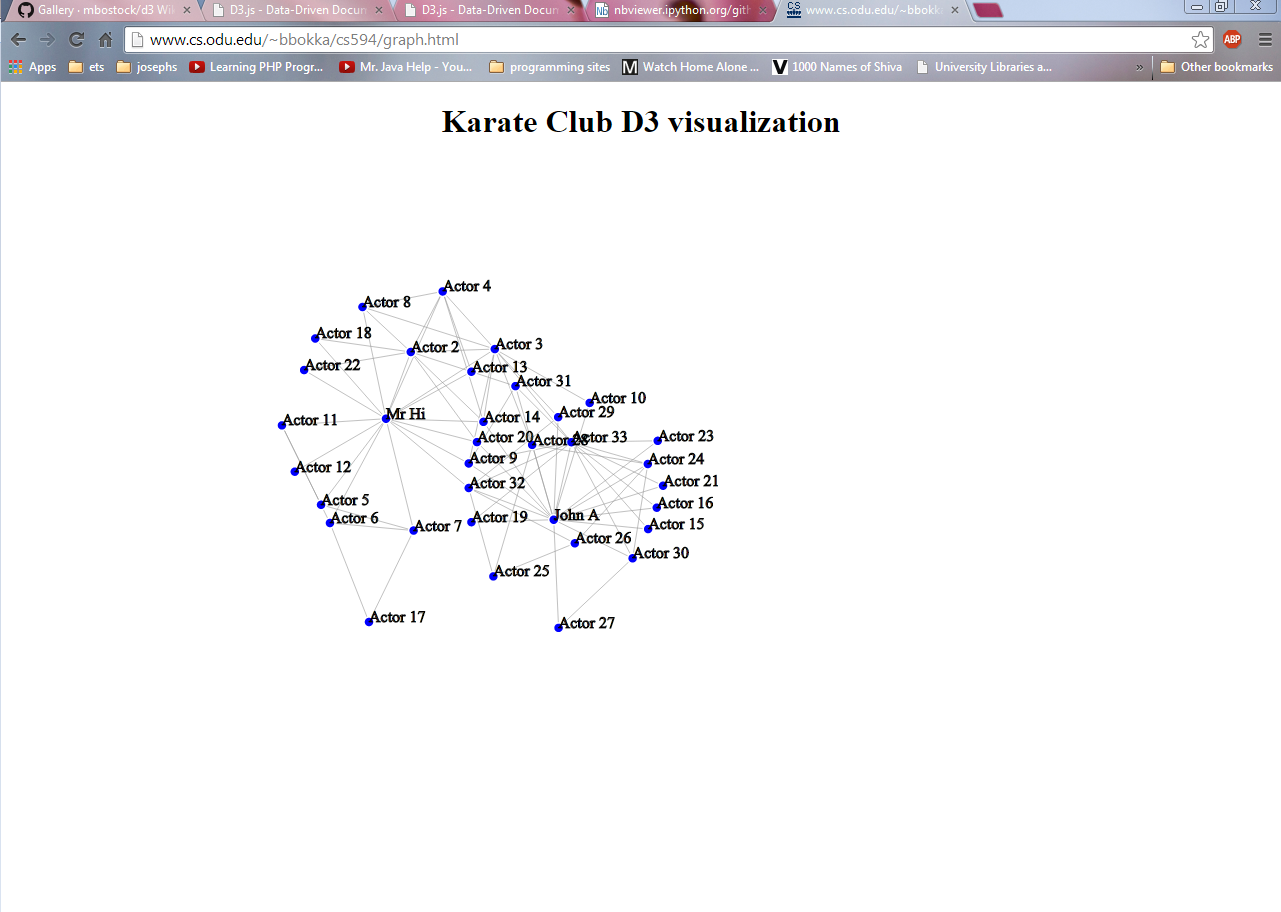
\includegraphics[scale=0.6]{../beforeSplit}
\centering
\caption{screen shot of the karate club}
\label{fig:before split}
\end{figure}
\newpage

\begin{figure}[ht]
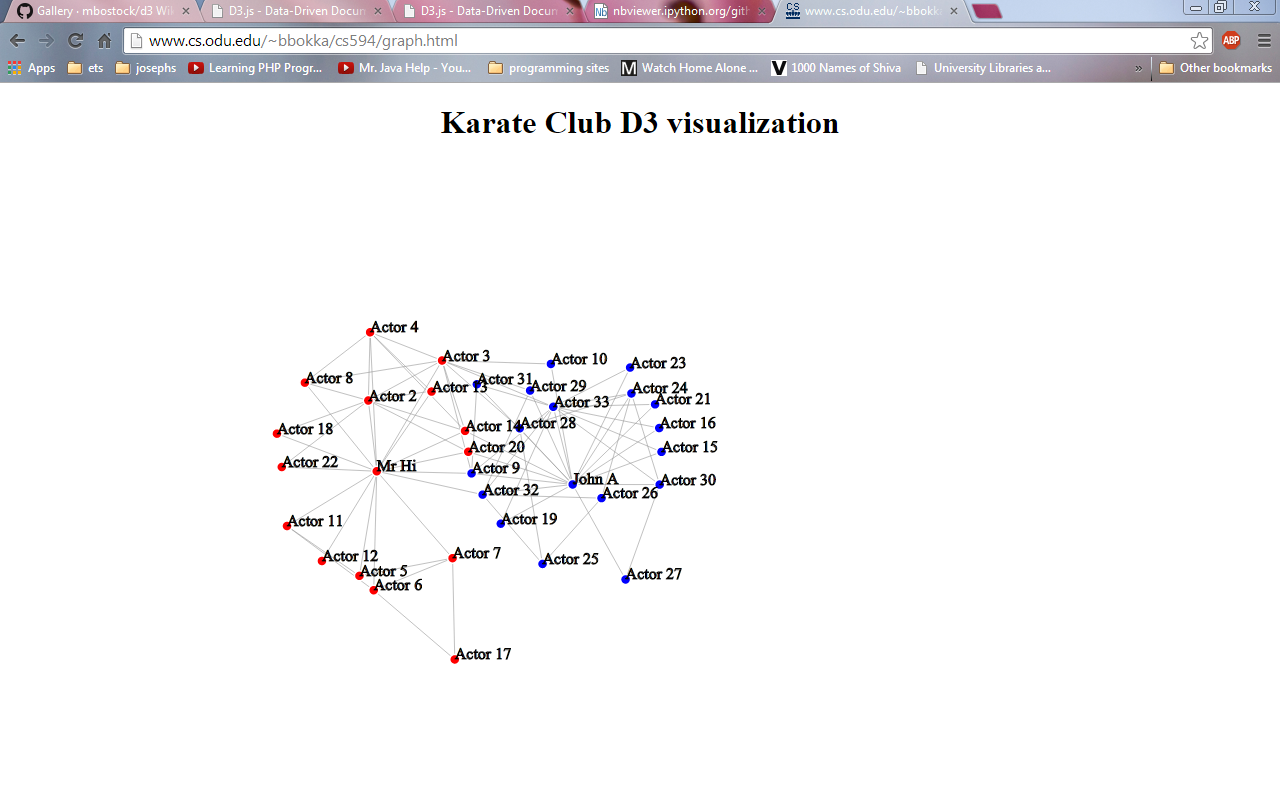
\includegraphics[scale=0.6]{../splitHighLlight}
\centering
\caption{screen shot highlighting the two groups}
\label{fig:after split}
\end{figure}
\newpage
%-----------------------End Question 1----------------------------
%------------------------------------------------------------------
%Bibilography
%------------------------------------------------------------------
\bibliographystyle{plain}
\bibliography{A7_report}
\cite{*}

\end{document}